\label{sec:coreference}

Our current work has primarily focused on event coreference resolution.

\section{Initial Approaches}
Our initial approaches were unsuccessful but largely informative: we tried modelling all mentions (cross-document) at the same time, in a \textit{mention-pair} manner.  Given $N$ mentions in a given topic, we evaluated $\frac{N*(N-1)}{2}$ mention pairs, with the aim of predicting which were coref or not (i.e., a 0 or 1 prediction).  Approximately 1 out of every 15 mention pairs are actually co-referenced (gold truth).  Our supervised, classification modelling attempts included using various LSTM and SVM approaches.


\textbf{LSTMs:} The LSTM approaches were based on the fact that if we let $m_{i-1}$ represent the word immediately before mention $m_{i}$ in the corpus, then $m_{i-1}$ will have high likelihood of predicting $m_{i}$.  Our idea was that if $m_{i-1}$ has high likelihood of also predicting mention $m_{j}$, then $m_{j}$ and $m_{i}$ might be coreference.  Our premise was that the likelihood of predicting each mention is directly correlated with each mention's likelihood of referring to the same event as $m_{i}$.  Despite many attempts, this never gave good results.  My conclusions were that:

\begin{itemize}
\item LSTMs are sensitive and are too close to memorizing the exact sequence of words, especially given the variance in our corpus
\item Our corpus' context varies too much and is not conducive to our premise.  For example, one sentence may be ``Barack Obama \textit{spoke} ... '' and another sentence may be ``The President, on Tuesday, \textit{spoke} ...''.  The word Tuesday is not likely to predict the word \textit{spoke}.
\end{itemize}

\textbf{SVMs:} Our SVM approach used a variety of commonly-used lexical features.  The performance exceeded the \textit{SameLemma} baseline.  However, difficulties included the class imbalance (too many negatives examples per positive example), along with the computational expense of training a proper kernel -- yielding the model intractable.

We also tried a generative, \textbf{topic modelling} approach, a la LDA with Gibbs sampling.  The underlying event was our latent variable: P(Event|Document) and P(Mention|Event).  Again, our performance barely rivalled the baseline of \textit{SameLemma}.  My conclusion was that predicting the number of latent classes (traditionally, number of topics) is too difficult and drastically affects the performance, especially since nearly half of all events only have 1 mention.

From these attempts, along with the two previously published works which have used a ECB+ corpus \cite{journals/tacl/YangCF15, Choubey2017EventCR}, I drew the following conclusions:
\begin{itemize}
\item an event-level model is not ideal, since it is inappropriate to predict how many unique events exist
\item negative sub-sampling is critical
\item most importantly, predicting within-document links first is critical and easier, as there are fewer mentions, and it serves as a stepping stone before considering links across all documents.  Then, one can use these predicted within-document clusters to merge with other within-doc clusters that reside in other documents. 
\end{itemize}

\section{CCNN: Conjoined Convolutional Neural Network}
Conjoined Neural Networks (a.k.a. Siamese Networks) were first introduced by Bromly and LeCun \cite{SiameseNet} for the task of determining if two signatures were from the same person or not.  Specifically, Conjoined Networks are two identical neural networks, each of which accepts distinct inputs, which are joined by a single loss function over their highest-level features.  The loss function computes a similarity score (e.g., euclidean distance) for an input pair.  The networks are said to be conjoined because they share the same weights and thus work together as one network that learns how to discriminate.  The benefits of tying the weights are that it:
\begin{enumerate}
\item Ensures that similar inputs will be mapped appropriately, otherwise, they could be mapped to hidden representations that are dissimilar from their input representations; and
\item Forces the network to be symmetric. If we abstractly represent the Conjoined Network as a function, then:
$CCNN(f_i,f_j) \equiv CCNN(f_j,f_i)$.  This is critical, as the CCNN's similarity function should be independent of the ordering of its input pair.
\end{enumerate}

Last, Conjoined Networks have been shown to perform well in low-resource situation \cite{Koch2015SiameseNN}.  This is ideal for our task, as it is highly likely that at test time we encounter event mentions that are out-of-vocabulary (OOV).  We desire our model to discriminately learn the relationships of input mentions, rather than exclusively relying on the input values themselves.  Likewise, we choose to use a Convolutional Network due to:
\begin{enumerate}
\item their power in learning sub-regions of features and the relations thereof, and
\item their recent advances in many NLP tasks \cite{DBLP:conf/emnlp/Kim14,DBLP:conf/acl/GehringAGD17,DBLP:journals/corr/YuV17}.
\end{enumerate}

\subsection{Input Features}
\label{sec:features}
Since our CCNN needs each mention to be represented exclusively by its own input, we used none of the relational features\footnote{We also experimented with extending our CCNN model by adding relational features as a merged-layer at the highest neural level.} that are common in other coreference systems (e.g., SameLemma, Jaccard similarity of mentions' context, shared WordNet parents).  We used Stanford CoreNLP \cite{manning-EtAl:2014:P14-5} to extract the following features, which we thoroughly tested in different ways:
\begin{itemize}
  \item \textbf{Part-of-Speech:} LSTM-learned POS embeddings; and 1-hot representations.
  \item \textbf{Lemmatization}: Lemmatized each token and represented it by pre-trained GloVe \cite{pennington2014glove} word embeddings.
  \item \textbf{Dependency Lemma:} we represent the dependent parent/children of each token via their aforementioned lemma embeddings.
  \item \textbf{Character Embeddings:} each token is represented as a concatenation of its character embeddings.
  \item \textbf{Word Embeddings:} pre-trained GloVe word embeddings.
\end{itemize}
We account for mentions' having varying token lengths by summing their tokens in place, thus representing each mention as a fixed-length vector.

\subsection{Architecture}
We define the full embedding for a given token $t$ as $t_{emb} = t_{f_{1}} \oplus t_{f_{2}} \oplus \ldots \oplus t_{f_{n}},$ where $\oplus$ represents vector concatenation and $t_{f_{i}}$ represents a specific input feature vector.

Naturally, we may want to convolve over the context of mention $m$, too, by including the $N$ words before and after $m$.  Thus, our input for mention $m$ is a matrix $M$, and a la Kim \cite{DBLP:conf/emnlp/Kim14}, we zero-pad unfilled windows.

\vspace{3mm}

Let $\textbf{M}$ represent the full matrix corresponding to mention $m$: $\textbf{M} \in \mathbb{R}^{(2N+1) \times d}$ and $\textbf{M}_{(i,j),(k:l)}$ represent the sub-matrix of $M$ from $(i,j)$ to $(k,l)$.

\vspace{3mm}

We define a kernel with dimensions $(h,w)$, where $h < (2N+1)$ and $w < d$.  This allows the kernel to operate on sub-sections of the embeddings.  The kernel has an associated weight matrix $\textbf{w} \in \mathbb{R}^{h \times w}$.  Starting at a given index $(i,j)$ within mention matrix $\textbf{M}$, a feature $c_{i}$ is defined as:
\begin{equation}
c_{i} = f(\textbf{w}^{T}\textbf{M}_{(i:i+h-1),(j:j+w-1)} + b)
\end{equation}
where $b \in \mathbb{R}$ is an added bias term.  The kernel runs over every possible sub-section of mention matrix $\textbf{M}$, yielding a feature map $\textbf{c} \in \mathbb{R}^{(2N-h) \times (d-w-1)}$

\vspace{3mm}

Since the network is comprised of two identical, conjoined halves, we sufficiently represent the architecture in Figure \ref{fig:ccnn} with just one half.  The Lambda function calculates the Euclidean distance of each half's univariate vector and emits a two-class softmax prediction regarding the likelihood of the two mentions being co-referent.

\begin{figure*}[h]
\centering
	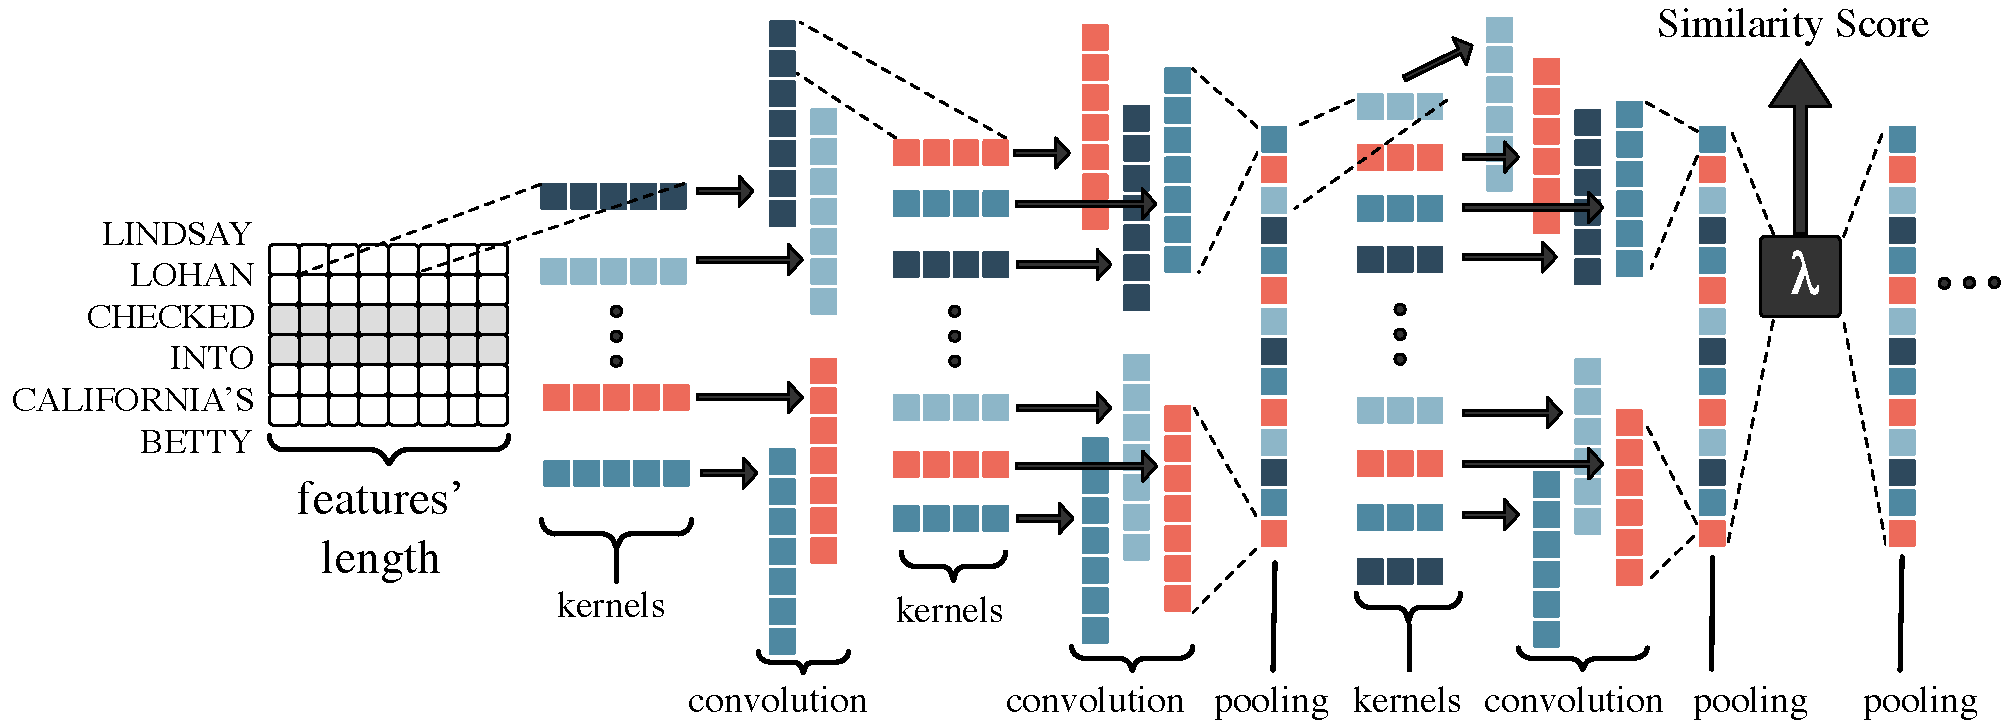
\includegraphics[width=1\textwidth]{graphics/architecture.pdf}
	\caption{One half of the Conjoined Convolutional Neural Network's Architecture.}
	\label{fig:ccnn}
\end{figure*}

\subsection{Loss / Optimization}
Our goal is to maximize discriminability of different event mentions, while enforcing features to be as similar as possible when they are of the same event.  Contrastive Loss, shown in Equation \ref{eq:contrastive}, is perfectly suited for this objective \cite{SchroffKP15,pmlr-v48-liud16}. Our training set has a strong class imbalance (most input pairs are not co-referent), so we down-sample to a 5:1 ratio of negative-to-positive examples.  We use Adagrad for optimization.
\begin{equation}
\begin{aligned}
L(&\hat{y},y)=\frac{1}{2N}\sum_{n=1}^{N}[(y)d^2 + (1-y)*(max(1-d,0))^2] \\
&\textnormal{where }d=\|y_{n}-\hat{y}_{n}\|_{2}
\end{aligned}
\label{eq:contrastive}
\end{equation}


%%%%%%%%%%%%%%%%%%%%%%%%%%%%%%%%%%%%%%%%%%%%%%%%%
%%%%%%%%%%%%%                5.   NEURAL CLUSTERING                %%%%%%%%%%%%%%%
%%%%%%%%%%%%%%%%%%%%%%%%%%%%%%%%%%%%%%%%%%%%%%%%%

\section{Neural Clustering (NC)}
\label{sec:clustering}
It is common practice for mention-pair models to first assign a probability score to every mention-pair, and then cluster with a different model.

\subsection{Existing Clustering Approaches}
\textbf{Agglomerative Clustering} is a simple but effective approach.  It first assigns each mention to its own singleton cluster.  Then, it repeatedly merges the two distinct clusters which contain the shortest-distance mention pairs.  Although this is a strong baseline, as seen in Yang, et. al. \cite{journals/tacl/YangCF15}, there are three main weaknesses:
\begin{enumerate}
\item One must define a stopping threshold $\alpha$.
\item Any given $\alpha$ hinges on the data being uniform across documents.  In reality, distances between mention-pairs could vary significantly between documents and topics.
\item Most significant, each cluster merge is based solely on two individual mentions, yet these mentions may not be representative of the cluster at large.
\end{enumerate}

\textbf{HDDCRP and Iterative-Folding Clustering} both contain the issue \#3 from above, as detailed in Sections \ref{sec:HDDCRP} and \ref{sec:Choubey}.

\subsection{Our Approach}
We aim to use the strengths of agglomerative clustering, while replacing its shortcomings.  We train a classifier to learn the most likely {positive cluster merge}, where the cluster is represented more holistically than a mention-pair basis.

Specifically, we learn a function $f(C_x,C_y)$ that predicts the likelihood of an appropriate, positive merging of clusters $(C_x,C_y)$. Let $d(m_i,m_j)$ be the mention-pair distance predicted by our CCNN model, where $m_i \in C_x$, and $m_j \in C_y$.  Function $f(C_x,C_y)$ is based on four simple features:
\begin{itemize}
  \item min-pair distance: $\min_{m_i,m_j} d(m_i,m_j)$
  \item avg-pair distance: $\frac{\sum_{m_i, m_j} d(m_i,m_j)}{\|C_x\|\|C_y\|}$
  \item max-pair distance: $\max_{m_i,m_j} d(m_i,m_j)$
  \item size of candidate cluster: $\frac{\|C_x\| + \|C_y\|}{\sum_{z}{\|C_z\|}}$
\end{itemize}

The first three features serve to better represent the cluster at large (issue \#3 from above).  For example, a given cluster $C_1$, when evaluated against two other candidate clusters $C_2$ and $C_3$, may have the same minimum mention-pair distance score with both $C_2$ and $C_3$  Yet, the average and maximum distance scores shed more light onto which cluster has more similar mentions. Cluster size represents the size percentage of our considered merge, relative to all mentions in our current set.  This may help prevent clusters from growing too large, and is not as vulnerable to issue \#2.

\subsection{Architecture}
We define $f$ as a feed-forward neural network\footnote{We used 1 hidden layer of 25 units, ReLU activation without dropout, and Adagrad as our optimizer.} which predicts the probability of a positive cluster merge, via a two-class softmax function.  Our loss function is weighted binary cross-entropy, to account for the class imbalance situation that most pairs of clusters should not be merged together.  

\subsection{Inference}
Our system will incrementally build up clusters, starting with each cluster having just one mention (in the within-document scenario).  Thus, it is important to train our Neural Clustering model on positive and negative examples of clusters in varying states of completeness.  Our gold truth data informs us which mentions are co-referent, but since there is no single canonical ordering in which mentions should become co-referent, we generate synthetic data to represent possible positive and negative examples of when clusters should be merged.

Specifically, for training, we generate a positive example by randomly sampling a golden cluster, followed by splitting the cluster into two random subsets.  The above four features are calculated for these two subsets of clusters, and the target output is a positive case.  Likewise, we generate negative examples by sampling random subsets from disjoint golden clusters.

At test time, we use Neural Cluster to evaluate every possible $(C_x, C_y)$ cluster pair in an easy-first manner.  That is, at each iteration, we merge only the $(C_x,C_y)$ pair that yielded the highest likelihood of a positive merge.  Then, we re-evaluate all pairs with our newly merged cluster, and repeat until the model no longer predicts merge.  Thus, unlike aforementioned models, we do not \textit{require} additional stopping parameters.

%%%%%%%%%%%%%%%%%%%%%%%%%%%%%%%%%%%%%%%%%%%%%%%%%
%%%%%%%%%%%%%%           6.   COREFERENCE SYSTEMS           %%%%%%%%%%%%%%%
%%%%%%%%%%%%%%%%%%%%%%%%%%%%%%%%%%%%%%%%%%%%%%%%%
\section{Our Coreference Systems}
\label{sec:coreference}

We use our CCNN and Neural Clustering (NC) models together to perform coreference resolution. The only differences between the within-document and cross-document scenarios are our data and evaluation metric, as described below.

\subsection{Training / Development / Testing Data}
We adhere to the same data splits as previous researchers, whereby the dev set is topics 23-25, and the test set is topics 26-45.  Traditionally, topics 1-22 are used as training.  However, since our NC model relies on our CCNN's predictions, we remove topics 19-22 from the training set and instead use them as dev sets for our NC models.  The complete details are provided in our Supplemental Materials document.

\subsection{Within-Document}
We train a CCNN model on mention-pairs which appear in the same document, and using its predictions on a held-out set, we train the NC to predict when to merge clusters.

\subsection{Cross-Document}
Cross-document resolution is a superset of the within-document task; it uses all coreference chains, regardless if mentions in a cluster were originally from the same document or not.  Our cross-document and within-document systems are identical, except: (1) we train a separate CCNN only on mention-pairs which are from different documents; (2) instead of initializing our clustering with all singleton clusters, we use our within-document NC predictions as starting clusters; (3) at each iteration, we only consider merging clusters $(C_x,C_y)$ if $C_x$ and $C_y$ contain mentions from disjoint sets of documents.  Our cross-document NC only uses cross-document mention pairs distances for its decisions.  Thus, cross-document merging will never merge two within-document clusters from the same document.

\section{Results}
As a recap, our research concerns three independent axis of investigation:
\begin{itemize}
\item \textbf{Features:} which features are most useful, and can we use few features?
\item \textbf{Mention-Pair Model:} how well does CCNN perform against a standard feed-forward neural network\footnote{Given two mentions $i$ and $j$, with corresponding feature vectors $f_i$ and $f_j$, their input to the Feed-Forward Neural Network is the vector $\|f_{i} - f_{j}\|$} (FFNN)?
\item \textbf{Clustering:} can we outperform Agglomerative via our Neural Clustering model?
\end{itemize}

Our metric is CoNLL F1 score, which is a clustering-based metric that combines the F1 scores of MUC, $B^{3}$, and $CEAF_{e}$, and we use the official scorer script (v8.01) \cite{Pradhan+etal:14a}.

\begin{figure*}[h]
\centering
	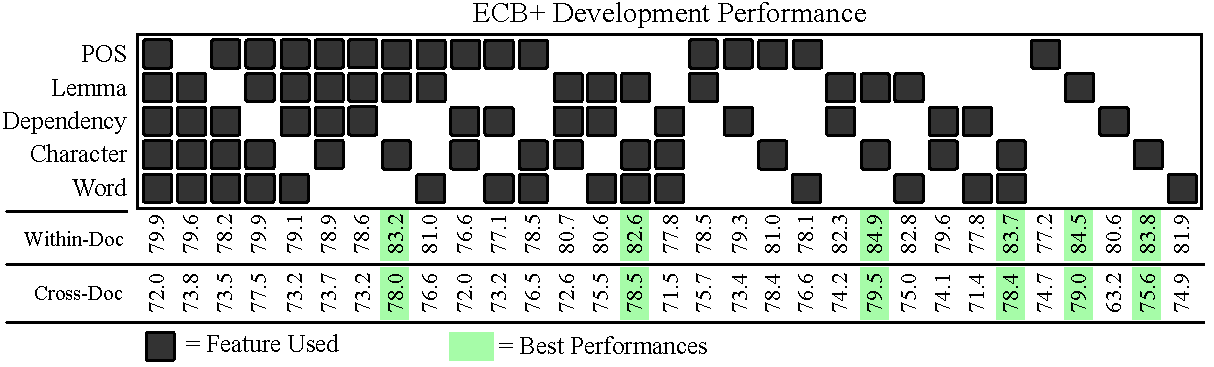
\includegraphics[width=0.82\textwidth]{graphics/features.pdf}
	\caption{The CoNLL F1 performance of our flagship CCNN + Neural Clustering system, using all combinations of features.}
	\label{fig:allfeatures}
\end{figure*}

We were interested in the five common, non-relational embedding features which are detailed in Section \ref{sec:features}: POS, Lemma, Dependency Lemma, Character, Word.  We tested all combinations of features on the Dev Set, and Lemma + Character Embedding yielded the best dev results (see Figure \ref{fig:allfeatures}).  Thus, our CCNN + Neural Clustering system used only these two features in its evaluation against other systems (see Table \ref{tab:others}).  

Our immediate evaluation measures the pairwise mention predictions.  As shown in Table \ref{} [TODO: make table], our CCNN model ourperforms the FFNN, SVM, and SameLemma baselines.

The final coreference results show that our CCNN model outperforms a FFNN, and that our Neural Clustering outperforms Agglomerative Clustering.  Figure \ref{} shows an example of where the aforementioned weaknesses of Agglomerative are improved by NC. [TODO: add figure demonstrating AGG VS NC examples.]  Further, when training and testing on gold mentions, we achieved CoNLL F1 scores of \textbf{81.2} and \textbf{72.4} for within-document and cross-document, respectively.  We denote these scores as the new baseline to which to compare future systems.

\begin{table*}[h]
\centering
\tabcolsep=0.15cm
\begin{tabular}{r|ccc|c|ccc|c|}
\cline{2-9}
& \multicolumn{4}{|c|}{Within-Document} & \multicolumn{4}{|c|}{Cross-Document}\\
\cline{2-9}
& \multicolumn{1}{c}{MUC} & B$^3$ & CEAF & CoNLL F1 & \multicolumn{1}{c}{MUC}& B$^3$ & CEAF & CoNLL F1\\
\hline
 \multicolumn{9}{|c|}{Test Set: ECB+ Gold Mentions} \\
 \hline
 \multicolumn{1}{ |c| }{SameLemma}& 58.3 & 83.0 & 75.9 & 72.4 & 84.2 & 68.2 & 48.0 & 66.8 \\
\multicolumn{1}{ |c| }{FFNN+AGG} & 59.9 & 85.6 & 78.4 & 74.6 & 77.7 & 69.9 & 50.1 & 65.9\\
\multicolumn{1}{ |c| }{FFNN+NC} & 60.7 & 86.7 &  79.4 & 75.6 & 74.9 & 67.8 & 56.3 & 67.0\\
\multicolumn{1}{ |c| }{CCNN+AGG} & 70.5 & 89.1 & 83.5  & 81.0 & 84.1 & 70.7 & 55.5 & 70.1\\
\multicolumn{1}{ |c| }{\textbf{CCNN+NC}}& 70.9 & 88.9 & 83.6 & \textbf{81.2} & 86.4 & 71.7 & 59.1 & \textbf{72.4}\\
\hline
\hline
 \multicolumn{9}{|c|}{Test Set: HDDCRP's Predicted Mentions} \\
 \hline
\multicolumn{1}{ |c| }{SameLemma}& 40.4 & 66.4 & 66.2 & 57.7 & 66.7 & 51.4 & 46.2 & 54.8 \\
\multicolumn{1}{ |c| }{HDDCRP}& 53.4 & 75.4 & 71.7  & 66.8 & 73.1 & 53.5 & 49.5 & 58.7\\
\multicolumn{1}{ |c| }{\textbf{CCNN+NC}} & 54.0 & 75.5 & 72.2  & \textbf{67.2} & 71.3 & 57.0 & 49.6 & \textbf{59.3}\\
 \hline
\hline
 \multicolumn{9}{|c|}{Test Set: Choubey's et. al. Mentions} \\
 \hline
\multicolumn{1}{ |c| }{SameLemma}& 48.8 & 66.7 & 65.1 & 60.2 &  68.1 & 53.3 & 47.2 & 56.2\\
\multicolumn{1}{ |c| }{Choubey}& 62.6 & 72.4 & 71.8  & 68.9 & 73.4 & 80.4 & 56.5 & 63.6\\
\multicolumn{1}{ |c| }{\textbf{CCNN+NC}} & 67.3 & 73.0 & 69.5  & \textbf{69.9}& 77.0 & 56.3 & 60.2 & \textbf{64.5}\\
 \hline
\end{tabular}
\caption{Comparison against other systems, while our models use only the Lemma + Character Embedding features.  FFNN denotes a Feed-Forward Neural Network Mention-Pair model.  AGG denotes Agglomerative Clustering.}
\label{tab:others}
\end{table*}

\textbf{Lemma Embeddings} were the most useful feature, followed closely by Character Embeddings.  Since \textit{SameLemma} has historically been a strong baseline, this is unsurprising.  

\textbf{Character Embeddings} were effective for the same reason String Edit Distance is often a strong feature: there tends to be a direct correlation between the textual similarity of mentions and their likelihood of being co-referent. Both random character embeddings and pre-trained ones yielded the same performance, suggesting that the power comes from the uniqueness of characters, not any \textit{meaning} conveyed in the characters.

Empirically, Lemma + Character Embeddings are complementary features; the semantic information conveyed within the lemma embeddings complement the syntactic information of character embeddings.  Related, POS by itself was a poor feature, but combining it with either Lemma or Character Embeddings offered strong results. 

Ideally, a classifier should learn how to combine all features such that the unhelpful ones are given no weight.  However, in practice, that is often extremely difficult, due to both the large parameter space and high entropy wherein some combinations of features seem to equally help as much as hurt.  Thus, we conclude that one should try to use the fewest features as possible for coreference resolution, then expand appropriately.

In all experiments, our results were inversely correlated with the amount of context our CCNN used.  That is, our best performance came when we used no context, only the mention words.  This agrees with the Choubey's, et. al. findings \cite{Choubey2017EventCR}.

\subsection{Comparison to Others' Systems}
\textit{SameLemma} has historically proven to be a strong baseline.  That is, anytime two mentions have identical lemmas, simply mark them as being co-referent.

Using the same mentions that were used by the HDDCRP and Choubey (Iteratively-Unfolding) systems, our flagship CCNN+NC system yielded the highest results, despite using few features.


\subsection{Error Analysis}
\textbf{False Positives} include mentions which are textually identical but not actually co-referent (e.g., \textit{placed} and \textit{placed}, which only differ in their direct objects).
\textbf{False Negatives} include abbreviations (e.g., \textit{i.r.} and \textit{injured reserve}) and colloquial phrases (e.g., The \textbf{casting} of Smith; (2) Smith \textbf{stepped into} the role; (3) was \textbf{handed the keys}).

[TODO: show actual examples]

Since our cross-document system relies on the within-document predictions, it is easy for errors to propagate.